\chapter{Progetto}
%ECHO algorithm per mandare dati formiche fine round a tutti i nodi.
%No lista di nodi conosciuti, formica non può venire mandata in nodi già visitati, non può venire mandata al nodo iniziale se ci sono archi a nodi non visitati (anche fittizi).
%\{deadlock, ANT, VISITED\_AGENTS\} <- messaggio in caso formica non possa muoversi su archi ``normali''.

%loopACO:
%    if userQueue =!= empty;
%        msg = pop.userQueue();
%        dealWithUser(msg);
%        for n in neighbourList
%            n ! msg;
%    if

In questo capitolo vengono presentati i moduli logici del sistema, gli algoritmi scelti, l'architettura ed i protocolli di comunicazione.
Infine, viene fornito un piano di sviluppo incrementale, partendo dalle funzioni di base.

\section{Architettura logica}
Il sistema da noi proposto è diviso in moduli, che differiscono per funzionalità e competenze, come segue:
\begin{itemize}
    \item Modulo ant colony: si occupa di gestire il funzionamento dell'algoritmo di ant colony optimization scelto, come verrà spiegato nella sezione \ref{sec:alg}. Questi metodi comprendono
    l'invio e la ricezione delle formiche, l'aggiornamento dei feromoni sugli archi;
    \item Modulo grafo: gestisce i metodi per l'aggiunta/rimozione di nodi dal grafo dei clienti e per l'aggiornamento dei pesi degli archi;
    \item Modulo utility: offre le funzionalità per lo scambio di informazioni tramite flooding con tutti i vicini di un nodo e per la scrittura a file di queste;
    \item Modulo ticket: comprende i metodi per il sistema di ticket, come descritto in \ref{sec:alg}, ovvero richiesta e rilascio di ticket per la modifica del grafo;
    \item Modulo API gestione clienti: interfaccia gli utenti ai metodi interni al sistema per la gestione dei clienti, questa comprende l'aggiunta e rimozione dei clienti e la modifica dei costi di spostamento;
    \item Modulo interfaccia grafica: è composto dai metodi per la visualizzazione tramite interfaccia web del grafo dei clienti e dell'approssimazione del percorso migliore;
    \item Modulo comunicazione: permette la comunicazione tramite messagi tra i moduli;
\end{itemize}
Tutti i moduli appena elencati sono utilizzati internamente dal sistema, tranne il modulo di gestione clienti, che viene usato dall'utente.

In figura \ref{fig:dep} sono presentate le dipende tra i moduli del sistema. Ogni ellisse rappresenta uno dei moduli sopraelencati. Una freccia da un modulo A ad un modulo B
indica che il primo dipende dal secondo. Ad esempio, il modulo ant colony dipende dal modulo comunicazione in quanto deve ricevere ed inviare formiche.

\begin{figure}
    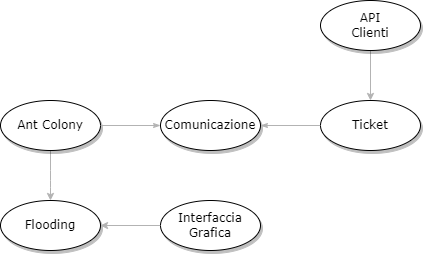
\includegraphics[width=\textwidth]{images/dependences.png}
    \label{fig:dep}
    \caption{Dipendenze tra i moduli del sistema}
\end{figure}
Describe the components of your systems: modules/objects/components/services.
For each component, describe the functionalities it implements, and by who is used.

\section{Protocols and algorithms}
Communication between components.  UML sequence diagrams go here.

Also, put here a detailed description of distributed algorithms used to solve specific problems of the project.

\section{Physical architecture and deployment}
Which nodes and platforms involved, and where each component is deployed.

\section{Development plan}
Since it is difficult to predict just how hard implementing a new system will be, you should formulate as a set of ``tiers,'' where the basic tier is something you’re sure you can complete, and the additional tiers add more features, at both the application and the system level.

\section{Algoritmi}\label{sec:alg}

\subsection{Algoritmo di Ant Colony Optimization}

\subsection{Flooding per la visualizzazione grafica}
Al fine di visualizzare il grafo ACO globale, tramite interfaccia grafica, è necessario che tutti i nodi pubblicizzino i propri
dati. È stato quindi pensato di utilizzare una variante asincrona dell'ECHO algorithm. 
Un nodo utente viene notificato da un nodo ACO quando finisce un round del percorso effettuato e propaga l'informazione tramite echo a tutti
gli altri nodi utente.

L'algoritmo si svolge come segue:
\begin{enumerate}
    \item il nodo utente iniziatore manda a tutti i suoi vicini i dati relativi al percorso ricevuto dal nodo ACO;
    \item ogni nodo ricevente, dopo aver archiviato i dati, inoltra il messaggio a tutti i nodi utente vicini, tranne quello da cui lo ha ricevuto;
    \item l'algoritmo termina quando ogni nodo ha ricevuto il messaggio.
\end{enumerate}

Usando un algoritmo asincrono come appena descritto, è possibile avere multipli flooding in contemporanea, senza dover aspettare che il precedente abbia finito.

\subsection{Aggiornamento del grafo dei clienti tramite ticket}
Per aggiornare il grafo dei clienti, è stato scelto di utilizzare un sistema a \textit{ticket}.
L'utente, per poter effettuare un aggiornamento, deve chiedere un ticket.
Verrà quindi mandato un messaggio al nodo ACO a cui è collegato, che lo inoltrerà al \textit{ticket master}.
Il ticket master risponderà quindi inviando il ticket, che l'utente potrà usare per fare richiesta di aggiornare il grafo.
Questo sistema serve per assicurare che gli aggiornamenti vengano fatti in ordine, ad esempio se un utente decide di aggiungere un nodo,
non deve essere possibile che un altro utente possa rimuoverlo prima che questo aggiornamento sia noto a tutti i nodi ACO.

\subsection{Elezione del ticket master}
Il ticket master è un nodo ACO che viene eletto tramite un algoritmo echo con extinction.
L'algoritmo esegue i seguenti passi:
\begin{enumerate}
    \item ogni nodo ACO fa da iniziatore per un nuovo echo, inviando il proprio ID a tutti i nodi vicini, rimanendo in idle;
    \item quando un nodo in idle riceve un echo (o lo trova in queue), confronta l'ID ricevuto con il proprio. Nel caso in cui l'ID ricevuto sia maggiore 
            di quello che ha correntemente memorizzato, rende il mittente il proprio genitore e aggiorna l'ID memorizzato 
            con quello appena ricevuto. Da questo momento, il nodo partecipa solamente all'echo iniziato dal suo genitore. 
    \item il nodo invierà l'echo a tutti i vicini tranne al genitore, aspettando una risposta dai vicini. 
            Appena ha ricevuto una risposta da tutti i vicini, invierà a sua volta una risposta al genitore;
    \item ad un certo punto, ogni nodo avrà iniziato a partecipare all'echo con ID maggiore, che sarà quindi l'unico correntemente in esecuzione;
    \item quando l'iniziatore di quell'echo riceve risposta da tutti i suoi vicini, viene eletto \textit{ticket master} e l'algoritmo di elezione termina.
\end{enumerate}
D'ora in avanti, i \textit{ticket} verrano richiesti al \textit{ticket master}.

Nel caso in cui un nodo fa richiesta di un ticket e non riceve una risposta entro una certa quantità di tempo, 
chiede a tutti i suoi vicini se hanno ancora il collegamento con il ticket master. Se riceve da tutti una risposta
negativa (o un timeout), si può quindi dedurre che il ticket master ha subito malfunzionamenti e viene iniziata una nuova elezione.

In figura \ref{fig:tm_ele} si può vedere un esempio di elezione. La topologia dei nodi è visibile in figura \ref{fig:tm_top}.

\begin{figure}
    \begin{subfigure}[b]{\textwidth}
        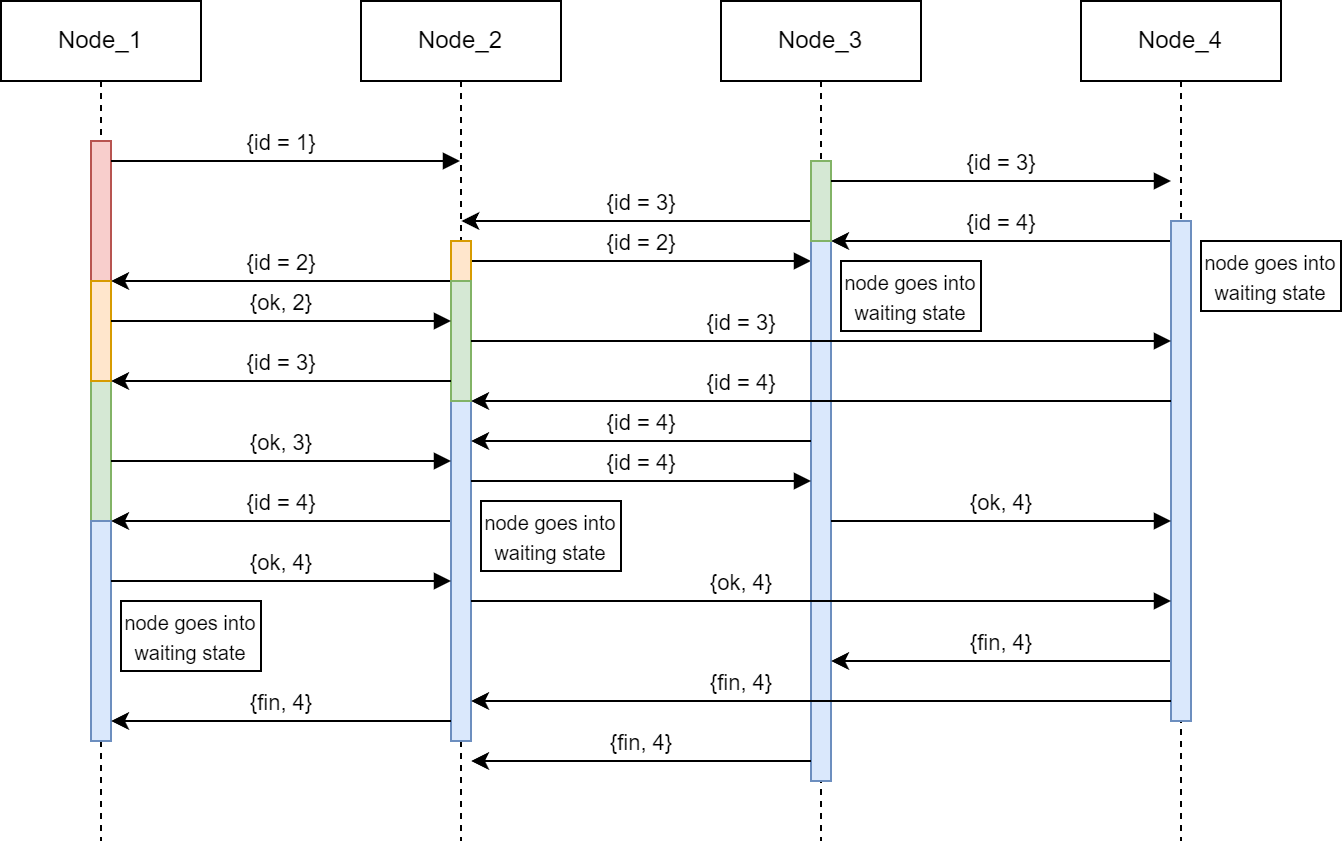
\includegraphics[width=1.2\textwidth]{images/ticket_master_election.png}
        \label{fig:tm_ele}
        \caption{Diagramma di sequenza dell'elezione del ticket master. I colori rappresentano i diversi echi, rosso per l'echo di ACO\_1, arancio per ACO\_2, verde per ACO\_3 e azzurro per ACO\_4.}
    \end{subfigure}
    \hfill
    \begin{subfigure}[b]{0.6\textwidth}
        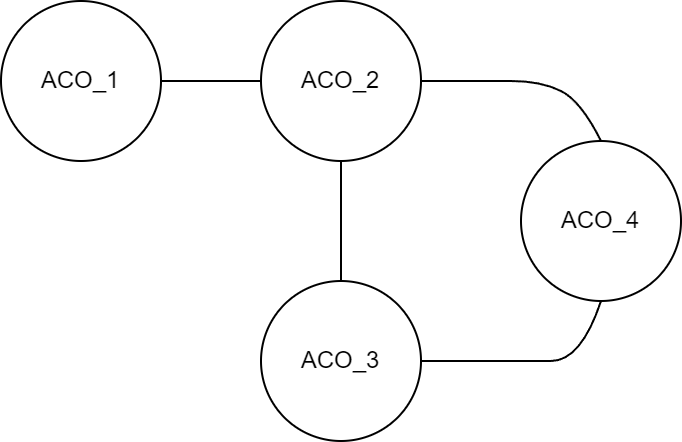
\includegraphics[width=\textwidth]{images/ticket_master_topology.png}
        \label{fig:tm_top}
        \caption{Topologia del grafo.}
    \end{subfigure}
    \caption{Esempio di elezione del ticket master.}
\end{figure}


\subsection{}